\documentclass[Rapport/Rapport_main.tex]{subfiles}
\begin{document}
\subsection{CoinDispenser}
\subsubsection{Hardwaredesign}
CoinDispenseren trengte en løsning på hvordan den kunne sortere og akseptere/avslå mynter som kom inn i systemet. Dette blir gjort med en statisk myntsorterings maskin som automatisk avslår alle mynter som ikke er 5kr. Den en er konstruert som en sklie som myntene sklir ned på med 2 huller, ett som er 27.5mm som er stort nåkk til at alle mynter som ikke er 5kr faller gjennom og ett hvor 5 kr myntene faller gjennom.

\begin{figure}[H]
    \centering
    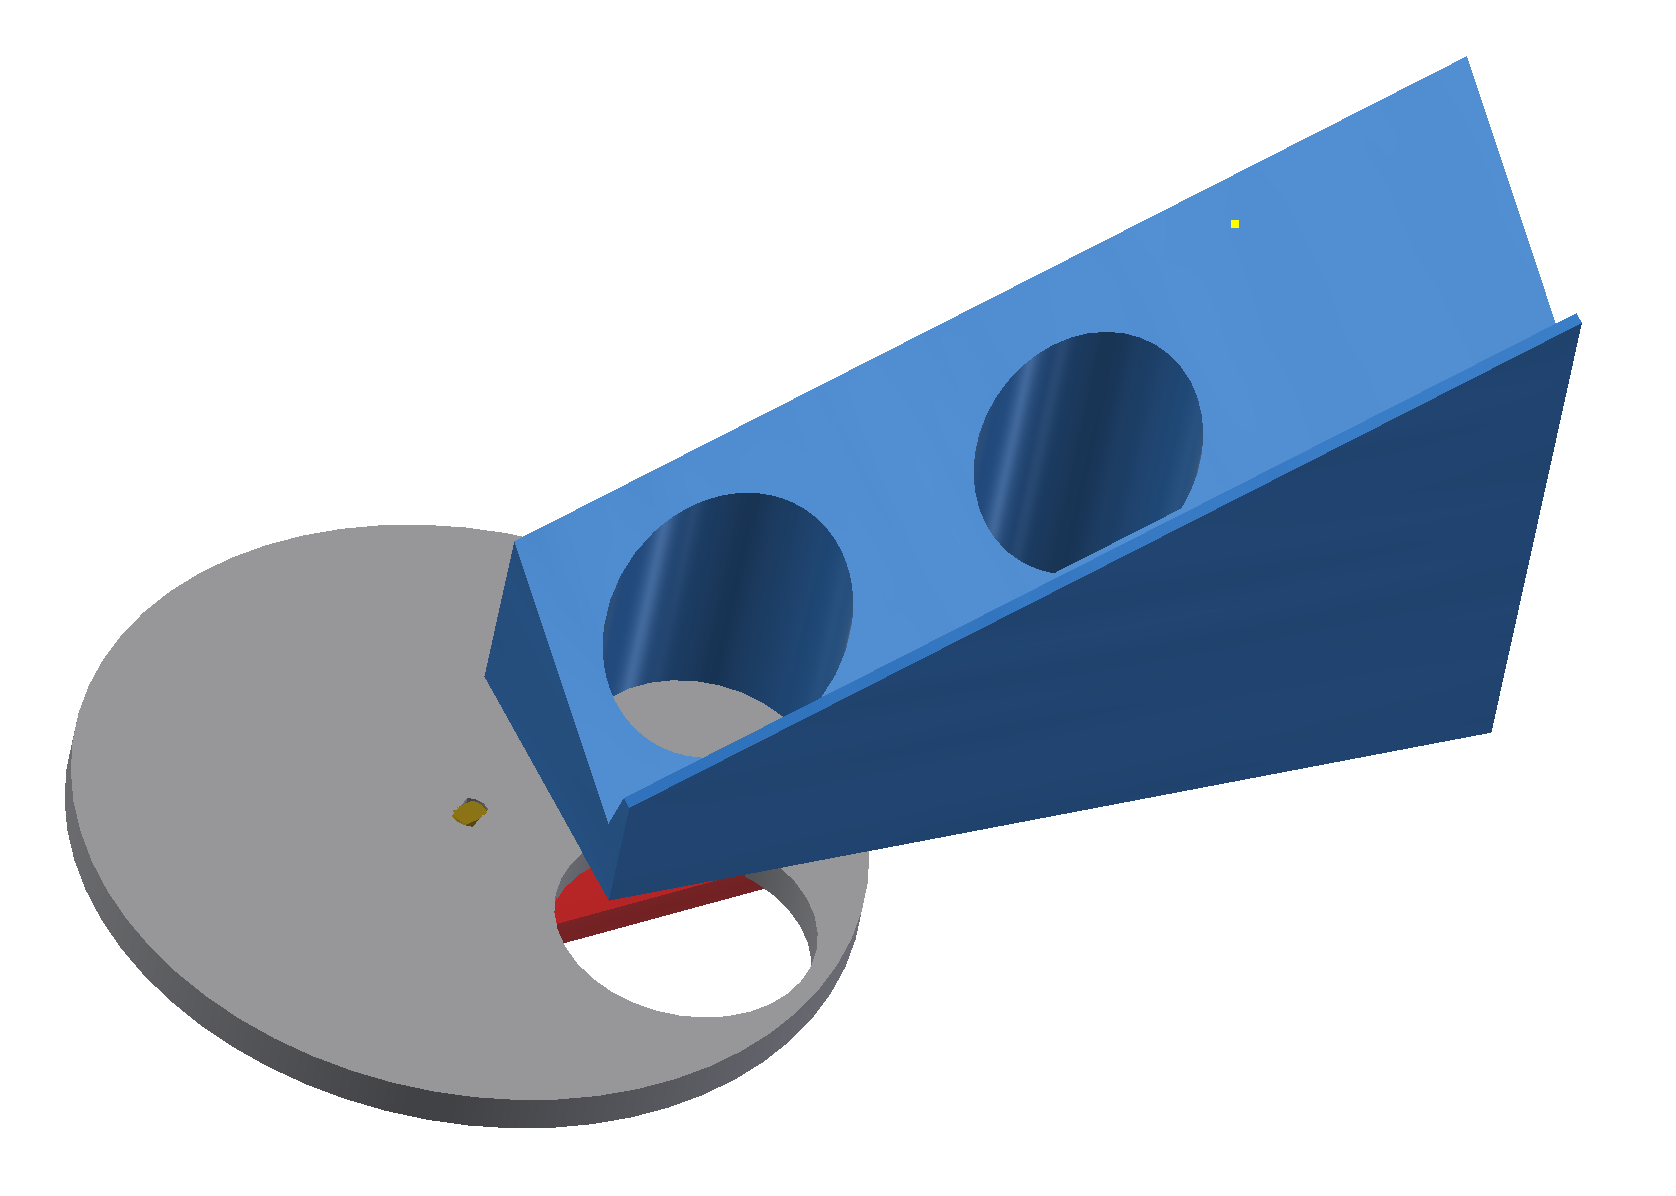
\includegraphics[width=\linewidth]{Rapport/BallDispenser/CoinDispenser/graphics/coinmaster.png}
    \caption{CoinDispenser CAD Model created in Autodesk Inventor}
    \label{fig:CoinCAD}
\end{figure}

Myntene er detektert ved av to metall plater som er nær hverandre, nå mynten faller ned på platen så kortsluttes koblingen og det sendes et interrupt til PSoCen.

\begin{figure}[H]
    \centering
    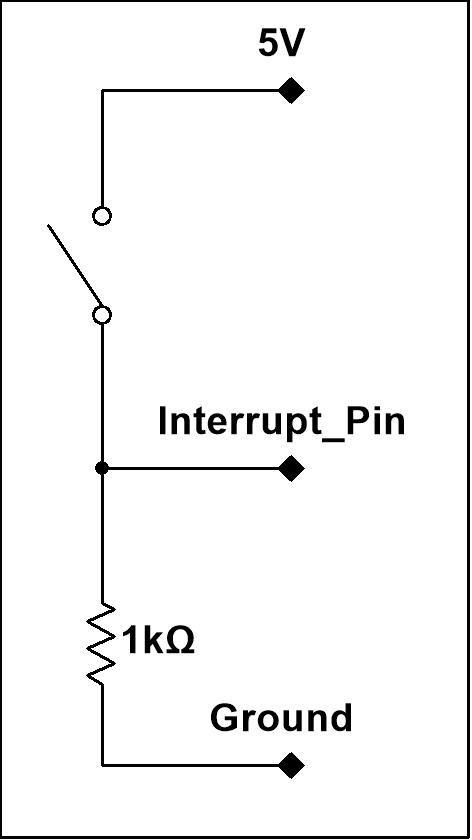
\includegraphics[width=0.3\linewidth]{Rapport/BallDispenser/CoinDispenser/graphics/CoinDispInterrupt.png}
    \caption{Coin Detection with shortcut setup}
    \label{fig:my_label}
\end{figure}

De sorterte mytene er akseptert eller avslått ved hjelp av en stepper motor koblet til en plate med et hull som ligger over metallplaten som er beskrevet over. Denne motoren er kontrollert av PSoCen og dreier med eller mot klokken avhengig av om den skal akseptere eller avslå myntene.

\begin{figure}[H]
    \centering
    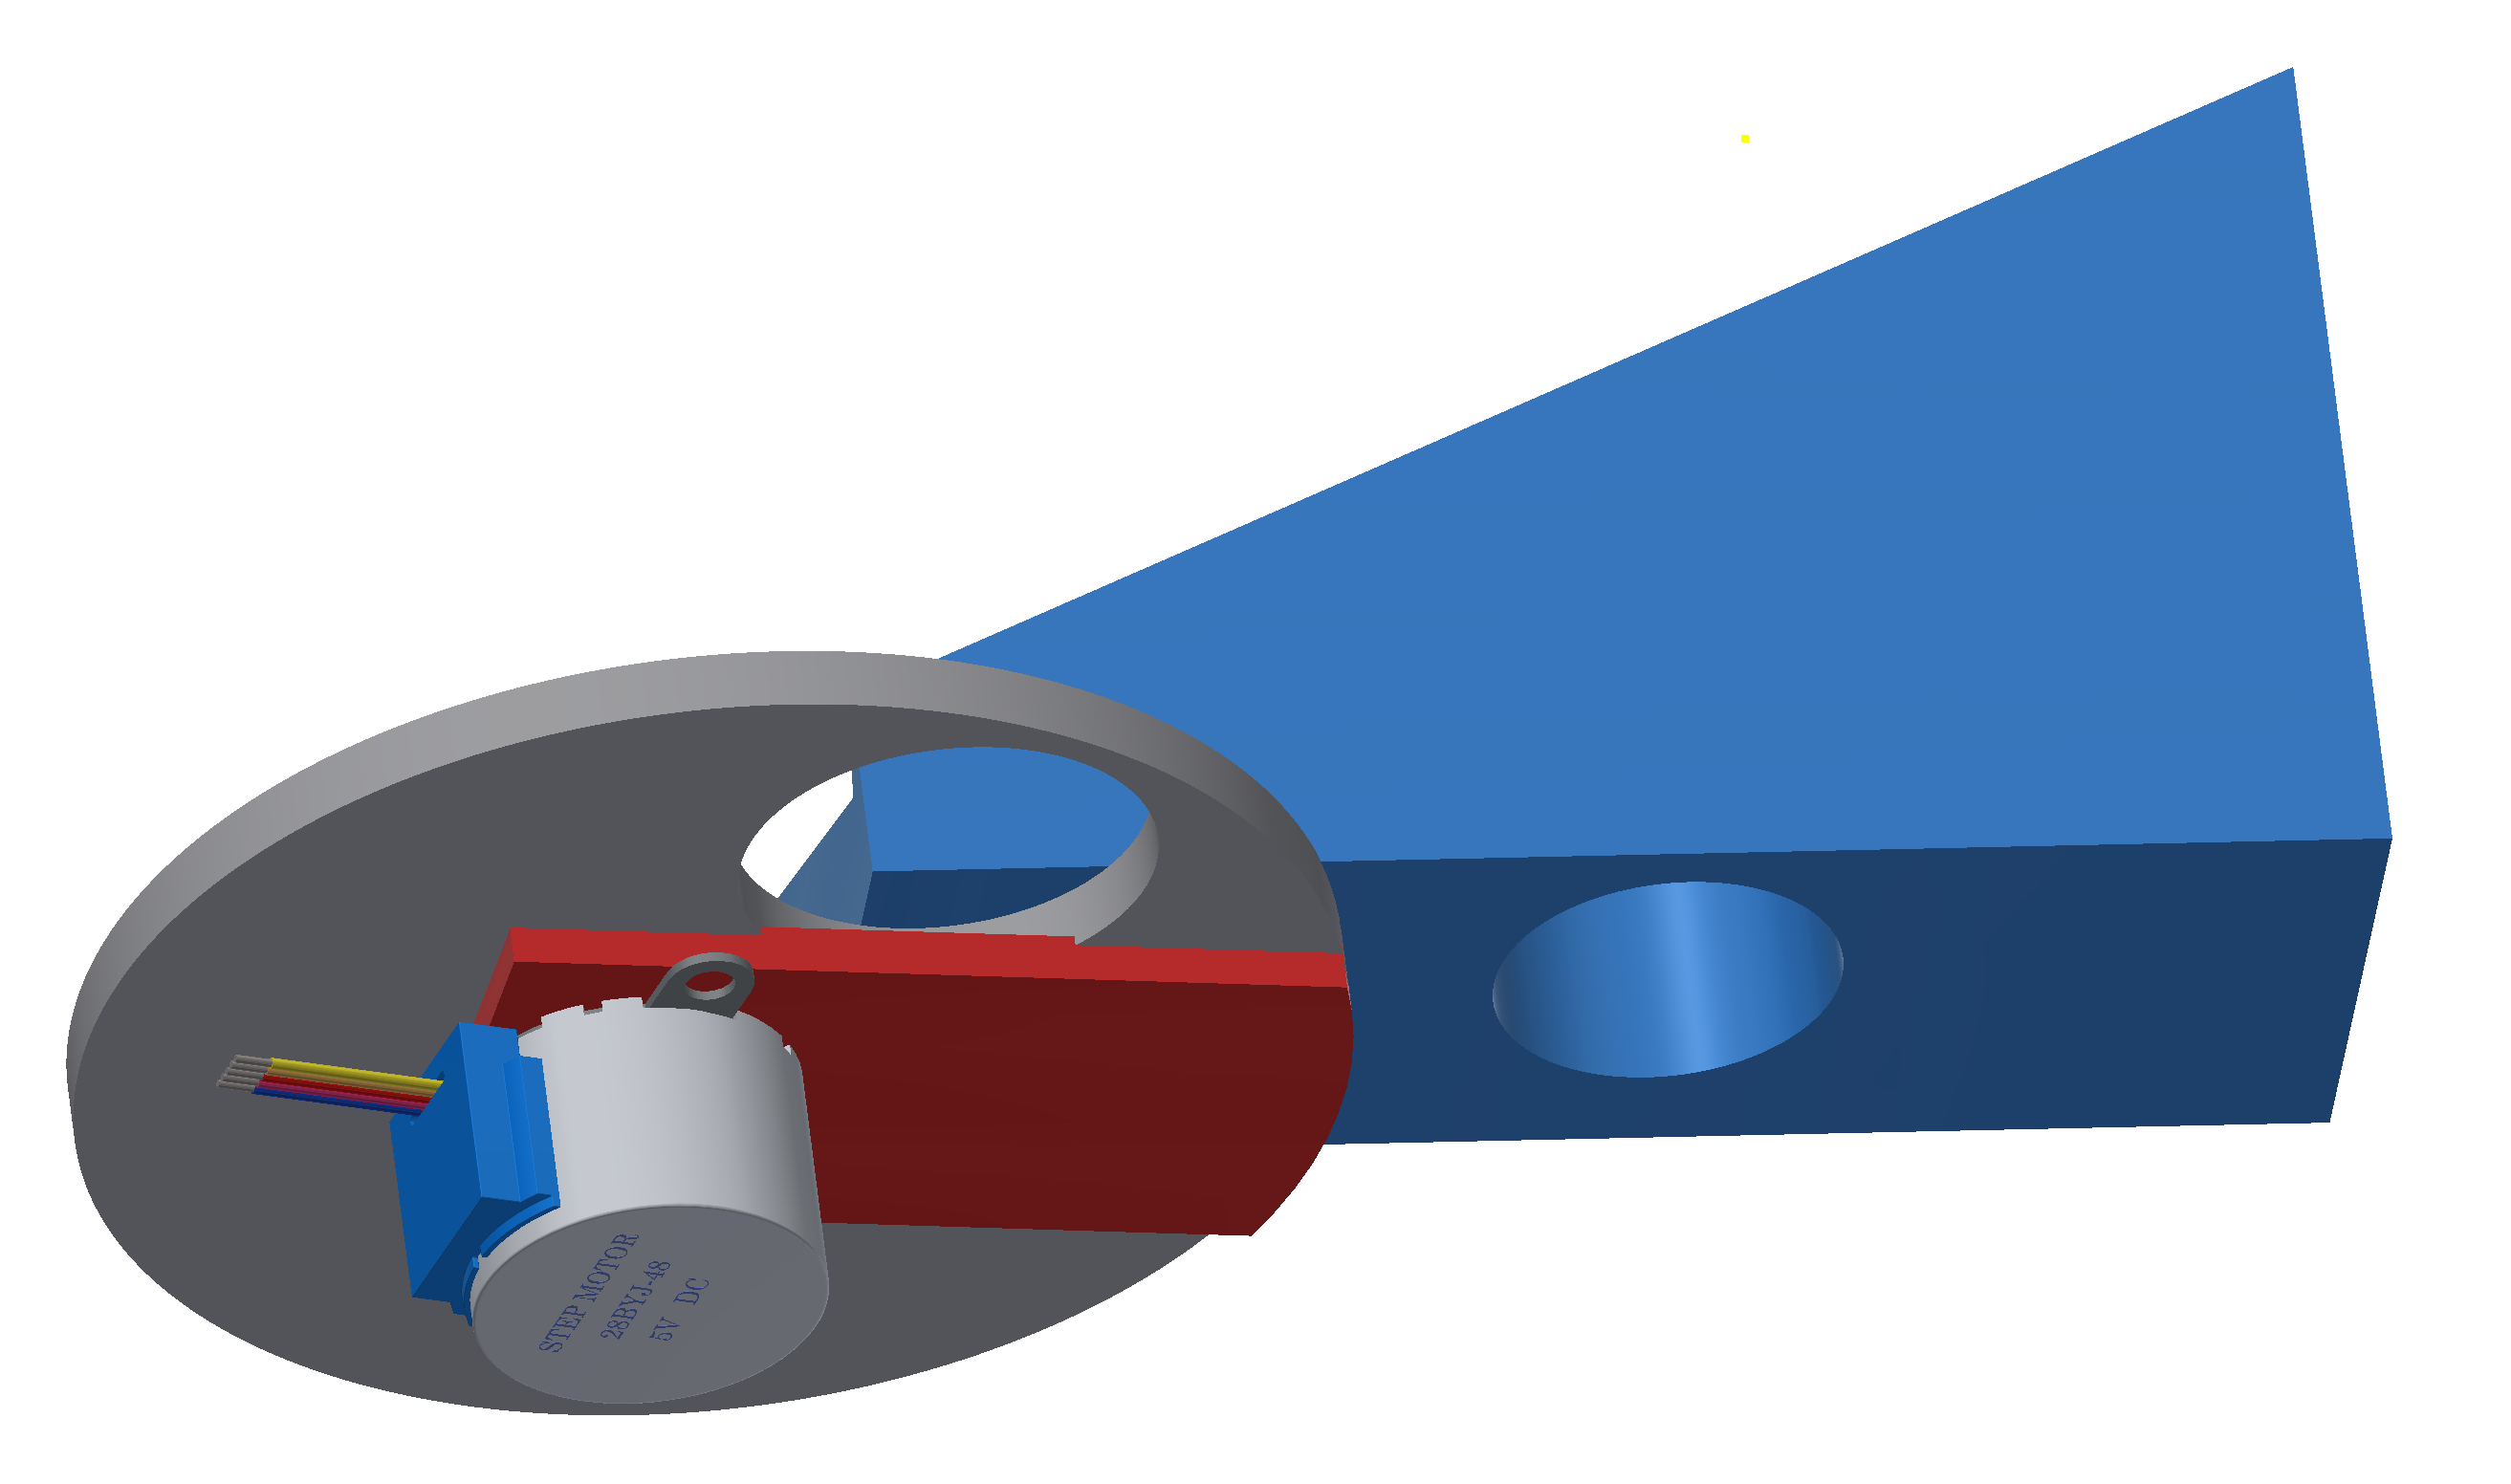
\includegraphics[width=1\textwidth]{Rapport/BallDispenser/CoinDispenser/graphics/coinmaster-under.png}
    \caption{CoinDispenser underside with steppermotor connected}
    \label{fig:my_label}
\end{figure}

\subsubsection{Softwaredesign}
\begin{figure}[H]
    \centering
    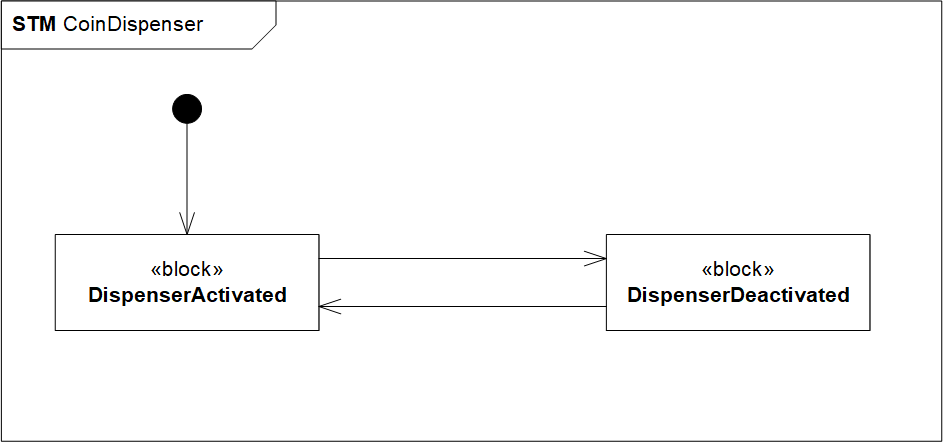
\includegraphics[width=1\textwidth]{Rapport/BallDispenser/CoinDispenser/graphics/CoinSTM.png}
    \caption{CoinDispenser State Machine}
    \label{fig:CoinSTM}
\end{figure}
I dette avsnitt beskrives designet for CoinDispenser classen på balldispenseren. Denne klassen skal kontrollere hardwaren til CoinDispenseren og sende beskjed til GameController hvis en mynt er innsatt. I grenseflate avsnittet i arkitekturen er en mer utdypende beskrivelse av disse beskjeder gitt. Den bruker I2C protokollen til å kommunisere med RPien. Classen bruker en external interrupt til å detektere mynter som kommer inn i systemet. Når en mynt detekteres kalles funksjonen HandleCoin som kan sees i arkitekturen, denne kaller funksjonene acceptCoin /rejectCoin etter som hvilket stadium CoinDispenser er i. Hvis systemet er i idle mode (DispenserEnabled) så aksepteres mynten og det sendes beskjed til GameController om at en mynt er akseptert. Hvis systemet er i playing mode (DispenserDisabled) så avvises mynten og systemet fortsetter å vente.
\subsubsection{Implementering}
Implementeringen av CoinDispenser er skrevet i C med bruk av PSoC Creator som er utviklings plattformen til PSoC. Ved å bruke PSoC Creator har vi tilgang til PSoCs komponent katalog.
\subsubsection{Modultest}
Modul testen til CoinDispenser ble gjennomført som en blackbox test med et unntak hvor vi må endre state fra enabled til disabled. Testen ble gjennomført ved a skli mynter ned sorterings sklien hvor de så lander på mynt deteksjons planten og observere om de blir detektert og håntert riktig i henhold til kravene. For tester av de individuelle komponenter og tabeller av resultatene refereres det til bilaget.\\
\end{document}